\documentclass{tufte-handout}

%\geometry{showframe}% for debugging purposes -- displays the margins

\usepackage{amsmath}

% Set up the images/graphics package
\usepackage{graphicx}
\setkeys{Gin}{width=\linewidth,totalheight=\textheight,keepaspectratio}
\graphicspath{{graphics/}}

\title{Regulation of Lipid Catbolism}
\author{}
\date{}  % if the \date{} command is left out, the current date will be used

% The following package makes prettier tables.  We're all about the bling!
\usepackage{booktabs}

% The units package provides nice, non-stacked fractions and better spacing
% for units.
\usepackage{units}

% The fancyvrb package lets us customize the formatting of verbatim
% environments.  We use a slightly smaller font.
\usepackage{fancyvrb}
\fvset{fontsize=\normalsize}

% Small sections of multiple columns
\usepackage{multicol}

% Provides paragraphs of dummy text
\usepackage{lipsum}

% These commands are used to pretty-print LaTeX commands
\newcommand{\doccmd}[1]{\texttt{\textbackslash#1}}% command name -- adds backslash automatically
\newcommand{\docopt}[1]{\ensuremath{\langle}\textrm{\textit{#1}}\ensuremath{\rangle}}% optional command argument
\newcommand{\docarg}[1]{\textrm{\textit{#1}}}% (required) command argument
\newenvironment{docspec}{\begin{quote}\noindent}{\end{quote}}% command specification environment
\newcommand{\docenv}[1]{\textsf{#1}}% environment name
\newcommand{\docpkg}[1]{\texttt{#1}}% package name
\newcommand{\doccls}[1]{\texttt{#1}}% document class name
\newcommand{\docclsopt}[1]{\texttt{#1}}% document class option name

\begin{document}

\maketitle% this prints the handout title, author, and date

\begin{abstract}
\noindent  This unit will discuss how lipids are oxidized and converted into energy.  Free fatty acids contain substantially more energy per molecule than either carbohydrates or proteins.  For more details on this process see Chapter 27 in Biochemistry: A Short Course available in reserve\cite{Berg2015}.
\end{abstract}

\tableofcontents

\pagebreak
\section{Learning Objectives}

\begin{itemize}
\item Explain how triglyceride breakdown into glycerol and free fatty acids is controlled in adipocytes by hormonal signals.
\item Explain how high carbohydrate diets affect fuel utilization, including effects on lipid fuel utilization.  Describe at an endocrine level how this is thought to occur.
\item Determine how much energy, in ATP equivalents, is released during the oxidation of a given fatty acid.  Be able to relate the energy content of a fatty acid, in general to its physical properties (length and saturation).
\item Explain the rate limiting steps of lipid oxidation.
\item Explain how ketone bodies are converted to ATP in non-hepatic tissues, and what governs this specificity.
\item Demonstrate an understanding of how how \textit{de novo} lipogenesis and $\beta$-oxidation are reciprocately controlled.
\item Describe how very long chain fatty acids are oxidized differently from long chain fatty acids.
\item Explain how odd-numbered fatty acids are catabolized, including the importance of vitamin B12 in this process. 
\item Evaluate the role of transcriptional regulation and long term adaptations to fatty acid oxidative capacity.
\end{itemize}


\section{Lipolysis Liberates Fatty Acids from Triglyerides}
Fatty acids are generally stored as triglycerides, and those triglycerides are primarily stored in adipose tissue.  There are two main sources of fatty acids, the dietary fatty acids liberated from chylomicrons by the activity of lipoprotein lipase\sidenote{This will be described in more depth in the lipid transport lecture}, and fatty acids liberated from adipose tissue\sidenote{A quantitatively small amount of lipids may be stored in liver (too much of this is called hepatic steatosis) and muscle (intramuscular triglycerides) tissues as well}.  This step, the conversion of triglycerides to fatty acids is known as lipolysis.

\newthought{In adipocytes the most potent activators of lipolysis} are catecholamines such as adrenaline and cortisol.  Adrenaline functions to rapidly activate adipocyte triglyceride lipolysis to glycerol and fatty acids via the activation of two enzymes, adipocyte triglyceride lipase (ATGL) and hormone-sensitive lipase (HSL).  These two enzymes work primarily on triglycerides and diglycerides respectively\sidenote{The last step, the conversion of monoacylglycerol to glycerol and a fatty acid, is catalyzed by monoacylglycerol lipase, an enzyme not thought to be regulated by hormones.}.  Via PKA-dependent signaling, both HSL and ATGL have increased rates of activity resulting in fatty acid release for use as energy in peripheral tissues.  Cortisol also increases lipolysis, potentially through several mechanisms, one of which is increasing the levels of ATGL, in a slower more permanent manner.  

\subsection{Carbohydrate Overfeeding and Lipid Utilization}

Insulin potently restricts adipocyte lipolysis.  The mechanisms of this are still not clear, but at least part of the actions of insulin are to inactivate HSL and ATGL by reversing the phosphorylation events caused by adrenaline.   States of insulin resistance such as type 2 diabetes means that insulin is less able to keep lipids in the adipose tissue.  Interestingly, studies where \emph{carbohydrates} are given in large quantities as part of overfeeding experiments lead to fat accumulation \citep{Acheson1988}.  This was originally thought to be due to activated \textit{de novo} lipogenesis, but more intricate studies showed that instead, the body was adapting to high levels of carbohydrates by sparing fat \citep{McDevitt2001} and that the level of lipogenesis was minimal.  This lipid sparing effect is the result of increased glucose oxidation and reduced lipolysis and $\beta$ oxidation.  This is a concept we have discussed several times already in this class, when one macromolecule is in relative excess, we tend to alter our metabolic pathways to use this for fuel\sidenote{Some examples we have already discussed include the inhibitory effects of Alanine on Pyruvate Kinase, Palmitoyl-CoA on Glutamate Dehydrogenase.}.  Of the multiple potential mechanisms for this lipid sparing effect, one is that carbohydrates induce a strong insulin response, which prevents lipolysis and results in lipids being trapped in adipose tissue.  This distinction is key to understanding how high carbohydrate diets relate to obesity.

\section{Fatty Acid Oxidation}

Fatty acid oxidation is important in many context, including during endurance exercise, and fasting.  It is particularly important in the heart where even under resting or elevated carbohydrate conditions, the majority of ATP is derived from fatty acid oxidation \citep{Neeley1974}.  Once fatty acids enter or are made available to the cell, they are quickly converted to "activated" forms known as acyl-CoA molecules\sidenote{The acyl refers to a generic fatty acid molecule, so the specific end product could be oleyl-coA (from oleate) or palmitoyl-CoA (from pamitate).}.  This is also the first step for triglyceride esterification, and consumes two ATP equivalents.  The enzymes that catalyze these reactions are known as Acyl-CoA Synthetases.  More details about these enzymes can be found in this recent review: \citep{Grevengoed2014}.

\begin{equation}\label{eq:acs}
Fatty Acid + CoA +  ATP \rightarrow AcylCoA + AMP + PPi
\end{equation} 

While there are several Acyl-CoA Synthetases, one in particular, ACSL1\sidenote{Abbreviated from Acyl-CoA Synthetase Long Chain Family Member 1, indicating a preference for long chain fatty acids} seems particularly important for fatty acid oxidation, as its genetic ablation in mice almost completely prevents fatty acid oxidation \citep{Ellis2011a}.  Interestingly, ACSL1 is present on the surface of the mitochondria in a physical complex with CPTI, the most important regulatory protein in fatty acid oxidation \citep{Lee2011l}.

\newthought{Mitochondria are key for fatty acid oxidation.}  Like most amino acid catabolism, fatty acid conversion to energy requires mitochondria.  However, unlike both pyruvate and most amino acids, for fatty acids the transport into mitochondria is the rate-limiting step.  This transport\sidenote{Which is more difficult than passive diffusion, due to the semi-insoluble nature of fatty acids} is controlled by the carnitine shuttle system.

\subsection{The Role of CPTI in Lipid Oxidation}

The carnitine shuttle system is a mechanism to get long chain fatty acids\sidenote{Short and medium-chain fatty acids can transport through the membranes freely, and therefore are not subject to this system.  This also means that they are not subject to regulation via malonyl-CoA-dependent inhibition.} through both the outer and inner mitochondrial membranes.  It comprises of two reactions and a transporter.  The reactions are overall energetically neutral, with the end products identical to the initial reactants.  The two reactions are catalyzed by Carnitine Palmitoyltransferase I (CPTI):

\begin{equation}
AcylCoA + Carnitine \rightarrow Acyl-Carnitine + CoA
\end{equation} 

and Carnitine Palmitoyltransferase I (CPTI):

\begin{equation}
Acyl-Carnitine + CoA \rightarrow AcylCoA + Carnitine
\end{equation} 

There is a transporter on the inner mitochondrial membrane called Carnitine Acyltransferase (CAT).  This transporter \emph{only} works with the carnitine conjugated fatty acids, so this transport system requires carnitine for its activity.  As we discussed in the non-protein compounds made from amino acids unit, carnitine can be made endogenously from the essential amino acid lysine.  Carnitine can also be obtained in the diet, with particularly high levels in red meat.


\begin{marginfigure}
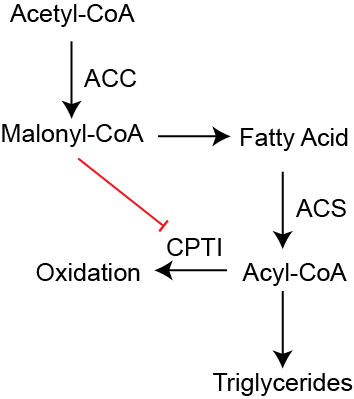
\includegraphics{figures/fatty-acid-oxidation.png}
\caption{Schematic of the regulation of fatty acid oxidation.  ACS indicates Acyl-CoA Synthetase, ACC indicates Acetyl-CoA Carboxylase.}
\label{fig:acc}
\end{marginfigure}


\newthought{Malonyl-CoA inhibits CPTI.}  This is the most important regulatory step in fatty acid oxidation.  If Acetyl-CoA Carboxylase is activated due to an excess of Acetyl-CoA, Citrate or insulin signaling\sidenote{Refer back to the lipid synthesis notes/lecture for more information} then there is a buildup of its product Malonyl-CoA in the cytoplasm.  This product potently inhibits CPTI \citep{McGarry1979}.  The result of this is to prevent fatty acid import and therefore fatty acid oxidation.  The activated fatty acids are then shuttled towards triglyceride synthesis rather than oxidation.  This regulatory process is illustrated in Figure \ref{fig:acc}.  The flip side of this inhibition is that when AMPK or PKA\sidenote{Via activation by adrenaline or glucagon for example.} are active, ACC is inhibited, Malonyl-CoA is reduced and CPTI is active.  In this way, energy demand or adrenaline can promote fatty acid oxidation.

\subsection{Lipid Oxidation in the Mitochondria}

Once the Acyl-CoA is inside the mitochondria, oxidation occurs through a series of enzymatic reactions.  These reactions proceed in a serial manner to extract one Acetyl-CoA at a time, removing two carbons each cycle.  The cycles consist of the following:

\begin{description}
\item [Desaturation] This generates a double bond at the $\Delta^2$ position of the fatty acid\sidenote{The Co-A group is attached at the carboxyl group, or the $\Delta^1$ position.}.  This step \emph{generates} one FADH$_2$ molecule.
\item [Isomerization] This transfers the electrons from this new double bond to a new ketone group on the  $\Delta^3$ carbon.  This step \emph{generates} one NADH molecule.
\item [Release] The first two carbons are now released as Acetyl-CoA by an enzyme called a thiolase.
\end{description} 

After one round, we are left with a fatty acid that is two carbons shorter, and have generated one Acetyl-CoA, one NADH and one FADH$_2$ that can be used as fuel.  For a saturated fatty acid such as palmitate (C16:0) this means that this cycle occurs \emph{seven} times\sidenote{Not eight, because the last reaction ends with two Acetyl-CoA molecules.}.

\subsection{Alternative Fatty Acid Catabolism}

Long chain, unsaturated fatty acids are catabolized in a very similar manner with one difference.  The first desaturation step introduces a double bond, but for unsaturated fatty acids the double bond is already present.  That means that during progressive oxidation, if an double bond is already present at the $\Delta^2$ of the now shortened fatty acid the first step is skipped, and FADH$_2$ is not generated.

\newthought{Odd-numbered fatty acids} after the last thiolase step, you end up with an Acetyl-CoA and a three carbon Propionyl-CoA\sidenote{Several amino acids, including Isoleucine, Valine, Threonine and Methionine also produce Propionyl-CoA}.  Propionyl-CoA is then converted to Succinyl-CoA by a three step reaction that in net consumes one ATP and requires Vitamin B12.  Succinyl-CoA is a component of the TCA cycle, and can be further oxidized generating one GTP and one NADH.  

\newthought{Very long chain fatty acids are first oxidized in the peroxisome.}  The Acy-CoA Synthetase with activity towards very long chain fatty acids\sidenote{Those with more than 22 carbons.} resides on teh peroxisomes.  Peroxisomes are membrane enclosed organelles that contain similar enzymes to those that perform $\beta$-oxidation in the mitochondria.  the major difference is that while these lipids are catabolised, there is not electron transport chain in peroxisomes, so no ATP is produced.  Instead electrons are transfered to peroxide, which is in turn converted to water and oxygen by the enzyme Catalase.  This process terminates with short and medium chain fatty acids that are released as acyl-carnitines where they travel to mitochondria for final catabolism and some energy production.

\subsection{Determining the Energy Content of a Fatty Acid}

Based on the series of reactions above, or each two-carbon unit released, one Acetyl-CoA, one NADH and one FADH$_2$ are released.  Added together this provides 14 ATP equivalents per two carbon units.  Therefore to calculate the ATP in a saturated fatty acid like palmitate (C16:0) we could do the following:

\begin{itemize}
\item Consume 2 ATP to activate the fatty acid (see the ACS reaction; \label{eq:acs}).
\item Take the fatty acid length, and subtract 2.  This is the number of fatty acid oxidation cycles.  For palmitate that is $\frac{16-2}{2}=7$.  For each cycle we generate 14 ATP units, for for palmitate there is $14 x 7 = 98$ ATP equivalents generated.
\item The remaining Acetyl-CoA adds another 10 ATP equivlents
\item The total ATP is then $98+10-2$ or 106 ATP equivalents.
\end{itemize}

For unsaturated fatty acids, you do not need to perform the desaturation step, so for each double bond there is one less FADH$_2$ generated than normal.  If we had a fatty acid that was 16:1 it would generate a total of 94.5 ATP equivalents.

\begin{margintable}
\centering
\caption{ATP equivalents of some fatty acids.}
\label{tab:fatty-acid-energy}
\begin{tabular}{@{}cl@{}}
\toprule
\textbf{Lipid} & \textbf{Net ATP} \\ \midrule
Butyrate (C4:0)           &  22                \\
Laurate (C12:0)          & 78                    \\
Palmitate (C16:0)          & 106               \\
Oleate (C18:0)          & 134              \\
Linoleate (C18:2)          & 131            \\ \bottomrule
\end{tabular}
\end{margintable}

\newthought{Generally this procedure explains two bioenergetic properties of fatty acids.}  Longer chain fatty acids have more energy than shorter chain fatty acids, and saturated fatty acids have more energy than desaturated fatty acids.  I have used the method above to calculate the ATP equivalents of several fatty acids in Table \ref{tab:fatty-acid-energy} to illustrate this point.  Don't try to memorize these, but rather spend some time practicing how to calculate the ATP-equivalents\sidenote{For even more of a challenge, try to calculate the net energy production from an odd-chain fatty acid.}.  After you have thought about how to calculate this, take a step back.  This is a lot of energy storage.  A triglyceride with three C16:0 molecules is catabolized to 318 ATP equivalents.  This is close to \emph{ten times} the energy storage of a fully oxidized glucose molecule (32 ATP).

\subsection{Ketolysis}

Ketone bodies are produced when there is excessive ATP, but insufficent TCA cycle intermediates in the liver.  These ketone bodies\sidenote{Primarily butyrate then acetoacetate; acetone is a terminal end product and cannot be used for energy.} can be converted back to Acetyl-CoA in non-hepatic tissues.  This specificity is due to the presence of an enzyme called 3-oxoacid CoA-transferase 1\sidenote{OXCT1, sometimes called succinyl-CoA-3-oxaloacid CoA transferase (or SCOT).}.  This enzyme catalyzes this reaction starting with Acetoacetate\sidenote{Butyrate can be interconverted to and from acetoactetate using up one NADH molecule for each acetoacetate generating, and using an NADH for the reverse reaction.}:

\begin{equation}\label{eq:oxct1}
Acetoacetate + Succinyl-CoA \rightarrow Succinate + Acetoacetyl-CoA
\end{equation} 

As a result this generates a single Acetyl-CoA molecule after a thiolase reaction.  This reaction is not cataplerotic because both Succinate and Succinyl-CoA are part of the TCA cycle.  However bypassing the Succinyl-CoA Synthetase step means that one GTP is not generated during normal TCA cycle progress.  Overall, an Acetyl-CoA that is released from the liver as butyrate costs the liver 3.5 ATP molecules \sidenote{1 ATP for the ATP-Citrate Lyase step, 2.5 ATP for the NADH used to generate butyrate}.  In the recipient tissue, that butyrate generates 6.5 ATP in net\sidenote{Generate 10 ATP from the TCA cycle oxidation of Acetyl-CoA, but using 1 NADH converting butyrate to acetoacetate; and 1 GTP skipping the Succinyl-CoA Synthetase step}.  Overall this means that this transport process means that the original Acetyl-CoA in the liver now results in 3 ATP equivalents rather than the 10 ATP if it remained in the liver.  Table \ref{tab:transport-processes} summarizes the energy costs of the three major transport processes we have discussed this year.  The \emph{inefficiency} of these transport processes is a cost to performance, but a benefit to generating negative energy balance for weight loss.

\begin{margintable}
\centering
\caption{Energy costs of the macromolecule transport processes discussed this year.  Refer to the gluconeogenesis notes for details about the Cori and Cahill cycles.}
\label{tab:transport-processes}
\begin{tabular}{@{}cl@{}}
\toprule
\textbf{Process} & \textbf{Net ATP Loss} \\ \midrule
Ketone Body Transport  &  -7 ATP  \\
Cori Cycle (Lactate)    & -6 ATP  \\
Cahill Cycle (Alanine)       & -15 ATP \\ \bottomrule
\end{tabular}
\end{margintable}

\section{Regulation of Fatty Acid Oxidation}

\subsection{Short-term Regulation}

As we described above, short term regulation is accomplished primarily through the ACC/Malonyl-CoA/CPTI system described in Figure \ref{fig:acc}.  Two other key regulatory systems to consider in the short term are the flux of fatty acids, either via the regulation of lipolysis, or the regulation of Lipoprotein Lipase activity\sidenote{Discussed in the lipid transport lecture.}.  Another regulatory mechanism that might not seem as apparent, is that when there is sufficient non-lipid fuel sources (for example an excess of carbohydrates or amino acids), there will be more Malonyl-CoA and therefore lipid oxidation.  Finally, recall that the products of fatty acid oxidation all require TCA cycle and electron transport chain activity.  Since the most important driver of the electron transport chain is energy demand, the final oxidation of all that Acetyl-CoA, NADH and FADH$_2$ will only occur if there is some energy demand.   Alternately, if there is insufficient TCA cycle intermediates\sidenote{For example due to cataplerosis in a liver undergoing substantial gluconeoegenesis.} the NADH and FADH$_2$ might be used for fuel but the Acetyl-CoA will undergo ketogenesis for transport for other tissues.

\subsection{Transcriptional Adaptations for Fatty Acid Oxidation}

\newthought{In terms of athletic performance,} increasing the ability to oxidize fatty acids is important for endurance athletes.  Highly trained athletes tend to have more mitochondria, and higher expression of enzymes such as Lipoprotein Lipase, CPT1, Acetyl-CoA Synthetase and enzymes of the TCA cycle.  One major regulator of these adaptations are a transcription factors called PPAR$\delta$ and PPAR$\alpha$.  In muscle tissues PPAR$\alpha$ and PPAR$\delta$  activates the transcription of several lipid transport and oxidation genes.  In liver tissues, a similar transcription factor, PPAR$\alpha$ upregulates many of the same genes\sidenote{Activation of PPAR$\alpha$ is a promising target to alleviate hepatic steatosis and non-alcoholic fatty liver disease (NAFLD), though they have not yet reached the clinic.} along with genes involved in ketogenesis \citep{Kersten2000,Badman2007}.  Both of these transcription factors are induced by elevated intracellular fatty acid levels \citep{Keller1993}.  The specific lnatural ligands for the PPAR transcritpion factors have been difficult to unambiguously identify, but PUFA's seem to play a key role in activating these transcription factors \citep{Forman1997}.  This is potentially one mechanism by which PUFA's alleviate lipid accumulation.

Interestingly, similar adaptations occur in the context of obesity, likely for the same reasons.  The major difference, is that in the absence of energy demand, lipids are only partially oxidized or end up stored as lipids in cells.  The buildup of stored, partially oxidized fatty acids is thought to play a role in the pathogenesis of insulin resistance, though the mechansims are not clearly defined.




\bibliography{library}
\bibliographystyle{plainnat}

\end{document}
